%% 
%% Copyright 2007-2024 Elsevier Ltd
%% 
%% This file is part of the 'Elsarticle Bundle'.
%% ---------------------------------------------
%% 
%% It may be distributed under the conditions of the LaTeX Project Public
%% License, either version 1.3 of this license or (at your option) any
%% later version. The latest version of this license is in
%%  http://www.latex-project.org/lppl.txt
%% and version 1.3 or later is part of all distributions of LaTeX
%% version 1999/12/01 or later.
%% 
%% The list of all files belonging to the 'Elsarticle Bundle' is
%% given in the file `manifest.txt'.
%% 
%% Template article for Elsevier's document class `elsarticle'
%% with numbered style bibliographic references
%% SP 2008/03/01
%% $Id: elsarticle-template-num.tex 249 2024-04-06 10:51:24Z rishi $
%%
\documentclass[preprint,12pt]{elsarticle}

%% Use the option review to obtain double line spacing
%% \documentclass[authoryear,preprint,review,12pt]{elsarticle}

%% Use the options 1p,twocolumn; 3p; 3p,twocolumn; 5p; or 5p,twocolumn
%% for a journal layout:
%% \documentclass[final,1p,times]{elsarticle}
%% \documentclass[final,1p,times,twocolumn]{elsarticle}
%% \documentclass[final,3p,times]{elsarticle}
%% \documentclass[final,3p,times,twocolumn]{elsarticle}
%% \documentclass[final,5p,times]{elsarticle}
%% \documentclass[final,5p,times,twocolumn]{elsarticle}

%% For including figures, graphicx.sty has been loaded in
%% elsarticle.cls. If you prefer to use the old commands
%% please give \usepackage{epsfig}

%% The amssymb package provides various useful mathematical symbols
\usepackage{amssymb}
%% The amsmath package provides various useful equation environments.
\usepackage{amsmath}
%% The amsthm package provides extended theorem environments
%% \usepackage{amsthm}
\usepackage{float}
%% The lineno packages adds line numbers. Start line numbering with
%% \begin{linenumbers}, end it with \end{linenumbers}. Or switch it on
%% for the whole article with \linenumbers.
%% \usepackage{lineno}

%% Added by author
% Allow long URLs in references to break at hyphens and other safe points.
\PassOptionsToPackage{hyphens}{url}
\usepackage{hyperref}
\hypersetup{
  pdftitle={Measuring NASA Science Plan Alignment with Scientific Consensus: A Case Study in Space Science},
  pdfauthor={Richard H. Witt, Anamaria Berea},
  colorlinks=true,   % true: colored links instead of boxes
  linkcolor=blue,   % color of internal links
  urlcolor=blue,    % color of external links/URLs
  citecolor=blue,   % color of citation links
  filecolor=blue,   % color of file links
  pdfborderstyle={/S/U/W 1} % underline links instead of boxes
}
\usepackage[table]{xcolor}    
\usepackage{booktabs}
\usepackage{colortbl}   
\definecolor{A6GreyBlue}{HTML}{5686AA}
\definecolor{A6GreyGrey}{HTML}{7d93a0}
\definecolor{A6LightGrey}{HTML}{E5E9EC}

\journal{Space Policy Journal}

\begin{document}

\begin{frontmatter}

%% Title, authors and addresses

%% use the tnoteref command within \title for footnotes;
%% use the tnotetext command for theassociated footnote;
%% use the fnref command within \author or \affiliation for footnotes;
%% use the fntext command for theassociated footnote;
%% use the corref command within \author for corresponding author footnotes;
%% use the cortext command for theassociated footnote;
%% use the ead command for the email address,
%% and the form \ead[url] for the home page:
%% \title{Title\tnoteref{label1}}
%% \tnotetext[label1]{}
%% \author{Name\corref{cor1}\fnref{label2}}
%% \ead{email address}
%% \ead[url]{home page}
%% \fntext[label2]{}
%% \cortext[cor1]{}
%% \affiliation{organization={},
%%       addressline={},
%%       city={},
%%       postcode={},
%%       state={},
%%       country={}}
%% \fntext[label3]{}

\title{NASA Science Alignment with Scientific Community}

%% Alternative title 1: if I add budget analysis
%%\title{Science, Policy, and Money: How Science gets funded in the United States}

%% use optional labels to link authors explicitly to addresses:
%% \author[label1,label2]{}
%% \affiliation[label1]{organization={},
%%       addressline={},
%%       city={},
%%       postcode={},
%%       state={},
%%       country={}}
%%
%% \affiliation[label2]{organization={},
%%       addressline={},
%%       city={},
%%       postcode={},
%%       state={},
%%       country={}}

\author[1]{Richard Witt\corref{cor1}}
\ead{rwitt4@gmu.edu}

\author[2]{Anamaria Berea}
% \ead{aberea@gmu.edu}

\affiliation[1]{organization={Computational and Data Sciences, PhD Student,George Mason University},
      addressline={4400 University Drive}, 
      city={Fairfax},
      postcode={22030}, 
      state={Virginia},
      country={USA}}

\affiliation[2]{organization={Computational Social Sciences, Associate Professor, George Mason University},
      addressline={4400 University Drive}, 
      city={Fairfax},
      postcode={22030}, 
      state={Virginia},
      country={USA}}

\cortext[cor1]{Corresponding author}

%%%%%%%%%%%%%%%%%%%%%%%%%%%%%%%%%%%%%%%%%%%%%%%%%%%%%%%%%%%%%%%%%%%%%%%%%%%%%%%%%%%
% Abstract
%%%%%%%%%%%%%%%%%%%%%%%%%%%%%%%%%%%%%%%%%%%%%%%%%%%%%%%%%%%%%%%%%%%%%%%%%%%%%%%%%%%
\begin{abstract}
%% Text of abstract
The National Academies of Science, Engineering and Medicine (NAS) conducts Decadal Surveys which NASA uses to prioritize budget and future strategy. This paper investigates how science plans at NASA align with scientific community consensus identified in the Decadal Surveys. We used Natural Language Processing (NLP) to compare these Surveys and NASA science plans, by highlighting similarities and discrepancies. We created a baseline of evidence based on a group of 4 Decadal Surveys from 2001 to 2007 and then we measured the similarities and dissimilarities between NASA science plans against this baseline. Alignment between science plans with baseline Decadal Surveys is shown to decrease over time (-0.001/year, p=0.024), which can indicate a potential decreasing effect of earlier Decadal Surveys on later science plans, a shift in scientific consensus, or a shift in operational realities. Science Mission directorate led science plans have higher median alignment ($p=9.9\times10^{-5}$) than NASA led strategic plans. 
\end{abstract}

%%Graphical abstract
\begin{graphicalabstract}
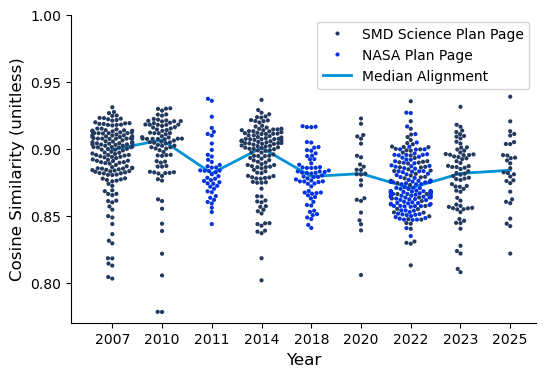
\includegraphics[width=0.9\textwidth]{SWARM_ALL.png}
\end{graphicalabstract}

%%Research highlights
\begin{highlights}
\item NLP-based semantic similarity to quantify NASA plan alignment with Decadal Surveys
\item Median alignment decreases by 0.024 similarity units from 2007 to 2025
\item SMD led science plans have 0.020 higher median alignment than NASA led strategic plans
\end{highlights}

%% Keywords
\begin{keyword}
%% keywords here, in the form: keyword \sep keyword
NASA science policy \sep Decadal Surveys \sep policy alignment \sep natural language processing \sep context embeddings \sep semantic similarity \sep science planning \sep space science

%% PACS codes here, in the form: \PACS code \sep code
\PACS 01.78.+p \sep 89.20.Dd \sep 01.75.+m \sep 89.70.Cf
% 01.78.+p (Science and government)
% 89.20.Dd (Space science policy and planning)
% 01.75.+m (Science and society)
% 89.70.Cf (Information and communication theory)

%% MSC codes here, in the form: \MSC code \sep code
\MSC 68T50 \sep 91B82 \sep 62P12 \sep 91F99
% 68T50 (Natural language processing)
% 91B82 (Statistical methods; economic indices and measures)
% 62P12 (Applications of statistics to environmental and related topics)
% 91F99 (Other social and behavioral sciences)
\end{keyword}

\end{frontmatter}

%% Add \usepackage{lineno} before \begin{document} and uncomment 
%% following line to enable line numbers
% \linenumbers

%% main text
%%

%%%%%%%%%%%%%%%%%%%%%%%%%%%%%%%%%%%%%%%%%%%%%%%%%%%%%%%%%%%%%%%%%%%%%%%%%%%%%%%%%%%
% Introduction and Literature Review
%%%%%%%%%%%%%%%%%%%%%%%%%%%%%%%%%%%%%%%%%%%%%%%%%%%%%%%%%%%%%%%%%%%%%%%%%%%%%%%%%%%
\section{Introduction}

NASA alignment with scientific community interests in science discovery is of major importance to the scientific community because it justifies federal funding of mission priorities, technology development, and theoretical research \cite{nasa_smd_hearing_2024}. Still, limited research has been conducted on this alignment with only two studies seeking to identify this relationship \cite{Trimble2011} \cite {pan2023seven_Decadals}. Trimble first conducted a retrospective review in 2011 by comparing what the Decadal Surveys asked for to what the scientific community received. Trimble found that roughly one third of requested facilities were completed with mostly federal funding within about 15 years. Pan and Trimble then conducted a followup review in 2023 expanding the review to roughly 60 years.  The survey reported 129 requests across Surveys 45 of which were federally funded within 15 years, 13 were funded within 15 years by mostly other sources. An additional 20 requests were eventually completed with federal funding, 11 were eventually completed with mostly other funding, and 38 were identified as never or very unlikely to be completed. The studies focus solely on Astronomy and Astrophysics. We aim to observe project alignment across all NASA Science Mission Directorates using natural language processing techniques. 

Creating a strategic plan for United States science discovery is a multi-agency, multi-year planning process. Two key corpora result from this planning process. The first corpus is U.S. National Academies of Science, Engineering, and Medicine (Academies) (NAS), which created the Decadal Surveys. The first Decadal Surveys were completed in 1964 in order to prioritize funding for astronomy projects that exceed individual agency budgets\cite{Academies2015_lessons}. The second corpus is composed of NASA planning documents authored at two different organizational levels. NASA Strategic Plans are products of the Office of the Administrator and establish agency goals and objectives\cite{WhiteHouse2021_space_priorities_framework}. SMD Science Plans which are products of NASA Science Mission Directorate and describe directorate-level science priorities, strategies, and implementation approaches.\cite{SMD_2025} In this paper we reefer to strategic and science plans collectively as NASA plans. NASA plans are used to define NASA project priorities while Decadal Surveys are used to identify scientific community interests.

% \subsection{Outline}

The remainder of this paper is structured as follows: Section~\ref{lit} describes Decadal Surveys, NASA Science Strategy, and introduces the concept of word embeddings. Section~\ref{data} details the source documentation used in the analysis. Section~\ref{meth} describes the methodology and rationale used to compare project priorities at NASA with scientific consensus using context embeddings.  Section~\ref{anal_results} provides the analysis and results from the documentation comparison. Finally Section~\ref{discussion} discusses the results and describes potential paths for future work. 

\section{Literature Review}
\label{lit}
\subsection{Decadal Surveys}

Decadal Surveys are a strategic guide for the planning and execution of United States investments in Science and Technology\cite{Academies2015_lessons}. The purpose of Decadal Surveys is to reach consensus on science priorities for the next decade while aligning with the executive branch initiatives and adhering to fiscal budget constraints. In 2015 the Space Studies Board at the Academies conducted a Survey of Decadal Surveys to capture lessons learned and best practices across 51 years of Decadal Surveys. The bulk of this section relies on this work except where otherwise cited \cite{Academies2015_lessons}.

Decadal Surveys are important to the entire scientific community. Survey chairs and committee members are accomplished scientists and engineers who are active leaders in their field from top institutions and universities throughout the world. A review of Decadal Survey committee and panel members reflects a distinguished roster of leaders in science and engineering. NASA and National Science Foundation (NSF) officials refer to the Decadal Survey recommendations as a blueprint or guidebook and individual research scientists refer to the Surveys as a "sword and shield": a sword for wining approval and shield against cancellation of federally funded programs. Two independent studies of Surveys in 2011 \cite{Trimble2011} and 2023 \cite{pan2023seven_Decadals} both found that around 71\% of projects identified in the Decadal Surveys are funded by either federal funds or other sources. The US federal government provided majority funding for 37\% of requested items within 15 years of the survey and 53\% of items overall. Other state, private, and foreign sources provided majority funding for 10\% of items within 15 years of the survey and 19\% of items overall. The remaining 29\% of items requested were identified as very unlikely to be built or put in operation. 

Stakeholders in the Decadal Surveys include many U.S. government agencies, departments, and private foundations that align with, or justify science funding by, Decadal Surveys such as the Alfred P. Sloan Foundation\cite{Sloan2021_decadal_private_funding} Gordon and Betty Moore Foundation\cite{Moore2017_hera_decadal_priority}, the Simmons foundation and the Heising-Simons Foundation\cite{NSF2023_advanced_simons_observatory}. NASA's Science Mission Directorate (SMD) is a typical and often central sponsor of the Decadal Surveys along with the NSF. Additional science community stakeholders in the Decadal Surveys include DOE, NOAA, and USGS. Congress, the Office fo Management and Budget, and other executive branch agencies use Decadal Surveys to evaluate budgetary plans.

This multi-agency, multi-stakeholder arrangement, as well as the considerable workload, high standards, and complexity of the task causes the process of conducting Decadal Surveys to be long and complex, typically lasting about 2 years from organizing the survey committee through delivery of the final report. The process starts with the Academies creating a statement of task for the committee to respond to. The Academies' Space Studies Board works with other standing committees at the Academies to select a Survey chair and committee of around 20 members. The Survey committee, with help from Academies staff, organizes panels and working groups around science themes such as outer or inner planets, stellar or galaxy evolution, climate variability and change, and solar wind-magnetosphere interactions; observational techniques such as X-ray or radio observations; facilities such as ground-based versus space-based telescopes; and subjects such as infrastructure, research grants, workforce diversity, applications, and graduate education. This freedom of organization allows for the culture of the scientific field and preference of the Survey organizers to mold the committee. The Surveys gather broad community input through public meetings, white papers, and direct presentations. The panels then create a ranked program of missions and activities based on science and observational capabilities specific to the panels area of responsibility. Panel priorities are then ranked across the field by the Survey committee. 

Independent reviews ensure scientific and fiscal rigor. Once panels and committees have completed their work, independent cost and risk evaluation is conducted for larger space missions and ground based facilities as mandated by the U.S. Congress. Evaluations are often contracted to private companies such as The Aerospace Corporation\cite{congress2008NASA}. The committee's report also undergoes an independent review to validate conclusions are supported and documented. The final report takes around 2 years to complete and provides a consensus vision of for its respective field.

Follow-up on Decadal Surveys requires multi-agency involvement. Once the Survey report is published the committee is disbanded. Post report stewardship is conducted by standing committees at the Space Studies Board through periodic reviews, which offer guidance to the agencies on Decadal programs. The NASA Advisory Council's Science subcommittees at the Academies follow NASA's progress. A congressionally directed midterm review of Decadal Surveys focus on agency progress to compare activities with Survey science goals is also conducted \cite{congress2005nasa}. The National Science Foundation receives input from the scientific community through proposals to it's various programs. The Department of Energy evaluates progress through extensive internal processes for energy related components of the Surveys while independent committees such as the Astrophysics Advisory Committee, provide advisory services on multi-agency projects.

Decadal Surveys serve as a national science strategy and are intended to inform science strategy at NASA and other federal agencies. 

\subsection{NASA Science Strategy}
NASA captures it's science strategy in NASA agency strategic plans and NASA Science Mission Directorate science plans. These plans are policy documents that turn national priorities, congressional direction, budget realities, and scientific-community guidance from decadal surveys into NASA's science objectives and portfolio balance. Instead of focusing on individual missions they set mission-development priorities. 

NASA relies heavily on Decadal Surveys to inform its science strategy. NASA's 2025 Presidents Budget Request states "SMD uses the recommendations of the National Academies' Decadal Surveys as important inputs in planning and prioritizing the future of its science programs." The same budget references Decadal Surveys 87 times, demonstrating NASA's focus on the Surveys to define science strategy \cite{NASA2025budget}. 

The Decadal Surveys are not the only input to NASA science strategy. The Office of the Chief Scientist (OCS) represents all of the scientific endeavors in the agency, ensuring they are aligned with and fulfill the administration's science objectives \cite{nasa_partnerships_2024}. International scientific consensus is also important, since two-thirds of SMD missions involve international partnerships \cite{nasa_smd_hearing_2024}. 
 
Science strategy is further refined by operational realities. The SMD Large Mission Study (LMS) Report lays out the most current Simplified Project Lifecycle available. This report identifies 7 Project Life-Cycle Phases, three of which occur prior to implementation and are therefore germane to the the project prioritization process. These 3 phases are: \emph{Phase Pre-A: Concept Studies}, \emph{Phase A: Concept and Technology Development}, and \emph{Phase B: Preliminary Design and Technology Completion}. During this process Decadal Survey recommendations are turned into decisions on mission architectures, preliminary requirements and budget estimates. In the Pre-Phase-A period, missions are not yet projects and focus is on quantifying science vs. cost and exploiting the range of solutions while maintaining dialog with Academy committees to ensure the intent of the Decadal Survey is honored. Once the decision authority determines the project is ready to transition into Phase A, the concept is determined to be executable. The concept begins to be developed into technology in Phase A and preliminary designs are completed in Phase B. Once Phase B is completed the concept becomes a project. \cite{NASA2020_LMS_study} \cite{wessen2013ConceptMaturity}.

The science strategy that results from this refinement process is defined in the NASA science strategy documents that are created.

\subsection{Word and Context Embeddings}
Information Retrieval has traditionally relied on concepts like the Bag of Words model\cite{harris1954}. In this approach text is represented into an unordered representation such as a sparse vector of term frequencies. These models were effective for keyword matching. However, they inherently disregarded word order or the surrounding context the word was used. 

To overcome the limitations of Bag of Words models modern word embeddings provide dense numerical representations of text. Embeddings can capture syntactic and semantic meaning for individual words \cite{mikolov2013_reps_of_words}, sentences \cite{reimers2019sentencebertsentenceembeddingsusing}, and documents \cite{wu_2018_doc_embeds}. These numerical interpretations, or word vectors, can be used to understand textual relationships mathematically. Essentially embedding turns text into a list of numbers known as a word vector. Each number describes some aspect of meaning or usage. Words like "planet" and "moon" have word vectors that are close together while unrelated words have word vectors that are farther apart. Embeddings can be compared using measures such as distance, similarity, or direction in a manner similar to comparing two dots on a scatter plot.
 
Embeddings work better with context. Early word embeddings were limited to a single global representation for each word. The ELMo model \cite{peters2018deepcontextualizedwordrepresentations} used context-dependent inputs to capture meaning across diverse contexts. ELMo was able to interpret words with polysemy thus beginning the era of Context Embedding models. These models represent words in the context of the surrounding words. Embedded context allows the model to distinguish the word "mission" in a space-science context from the same word in a religious context. Context-aware embeddings can be used to define meaning based on how the word is used. 

Context aware models have evolved significantly since ELMo and a are a core technology behind Large Language Models. BERT \cite{devlin2019bert_pretraining} added bidirectional encoding, GPT \cite{radford2018improving_GPT} added auto-regression prediction and BART \cite{lewis2019bart} combined these two innovations to increase performance on text generation tasks. Embedding models are used as an unsupervised stage prior to the supervised fine tuning stage for transformer based large language models since their inception \cite{vaswani2023attentionneed} and in current state of the art open source models \cite{grattafiori2024_llama3_herdmodels}.

Our research relies on OpenAI's \texttt{text-embedding-ada-002} model due to its favorable performance in document level search \cite{Aperdannier2024_embedding_search}. The model was released on December 15, 2022 \cite{openai2023ada_embeddings} as closed source. However, on January 24, 2022 OpenAI published Text and Code Embeddings by Contrastive Pre-Training \cite{neelakantan2022openAi_embeddings} indicating that \texttt{text-embedding-ada-002} is likely an evolution of this prior work using a contrastive objective on paired samples with relatedness evaluated by measuring cosine similarity.  Cosine similarity measures the direction, or angle, between word vectors.  More precisely it measures the the cosine of the normalized directional alignment between two word vectors. Cosine similarity was likely chosen by the OpenAI Contrastive Pre-Training team because it compensates for document size by length normalizing the vectors to unit vectors. We use it here for the same reason. By normalizing for document length we avoid errors prevalent in techniques that measure distance between vectors. Distance measures fail to recognize similar documents that differ significantly in length simply because words appear more often in longer documents.\cite{manning2008_introduction_ir}.

%%%%%%%%%%%%%%%%%%%%%%%%%%%%%%%%%%%%%%%%%%%%%%%%%%%%%%%%%%%%%%%%%%%%%%%%%%%%%%%%%%%
% Data
%%%%%%%%%%%%%%%%%%%%%%%%%%%%%%%%%%%%%%%%%%%%%%%%%%%%%%%%%%%%%%%%%%%%%%%%%%%%%%%%%%%
\section{Data}
\label{data}
\subsection{Decadal Surveys}
The National Research Council (NRC) of the Academies has conducted Decadal Surveys at approximately a 10 year cadence since 1964. Decadal Surveys typically require 2 years to complete each Survey \cite{Academies2015_lessons}. Until 2003, Decadal Surveys were focused on Astronomy and Astrophysics. However since then, Decadal Surveys are listed into the following 5 categories: Astrophysics, Planetary, Heliophysics, Earth, and a final category of Biological and Physical Sciences.

The purpose of Decadal Surveys is to reach consensus on science priorities for the next decade, while aligning with the executive branch initiatives and adhering to fiscal budget constraints. Science community stakeholders in the Decadal Surveys include NASA, NSF, DOE, NOAA, and USGS. Congress, the Office fo Management and Budget, and other executive branch agencies use Decadal Surveys to evaluate budgetary plans. Given the magnitude of impact of the studies, Survey committees consist of experienced, active, and accomplished leaders in their respective fields \cite{Academies2015_lessons}.

Decadal Surveys for this report were sourced directly from the National Academies Press website \cite{Academies_Decadal}. NASA also lists the most recent Decadal Surveys on it's Science Mission Directorate website \cite{NASA_Decadal}.

\subsection{Science Strategy}
NASA Science plans define NASA Science strategy and cross all 5 Decadal Survey categories to provide guidance for each division of the SMD. 

NASA Science plans have two distinct sources. Three of the plans in the corpus are created as NASA Strategic Plans, signed by the NASA Administrator, and seven are Science Mission Directorate (SMD) Science Plans, signed by the Associate Administrator of the Science Mission Directorate\cite{SMD_2007} \cite{SMD_2010} \cite{NSP_2011} \cite{SMD_2014} \cite{NSP_2018} \cite{SMD_2020} \cite{NSP_2022} \cite{SMD_2022} \cite{SMD_2023} \cite{SMD_2025}.

 NASA Science Mission Directorate has a web page devoted to science strategy containing SMD Science Plans, NASA Strategic Plans, and accompanying documentation for most years beginning in 2007 \cite{NASA_sci_strat}. 

 The divisions of the SMD closely align to the Decadal Surveys and consist of 6 divisions reporting to the Deputy Associate Administrator \cite{NASA_SMD}. Four of the divisions are represented in Table~\ref{tab:Decadals_used}. Joint Agency Satellite Division and Biological and Sciences Division are not mapped to the Decadal Surveys. Joint Agency Satellite has no corresponding Decadal Surveys and Biological and Physical Sciences first Survey occurs in 2011 after the first available science plan and was removed to avoid temporal leakage from science plans affecting Decadal Surveys.  

\subsection{Matching Surveys with Strategy to measure Context Similarity}
Four Decadal Surveys published between 2001 and 2007 were chosen to determine if Decadal Survey effects are observable on NASA Science Plans using semantic similarity.  This reduction has two effects on our data sample. First it reduces the data to points in time prior to the first NASA Science Plan analyzed in the report. Second it creates a sample that represents a cross section matching the scope of NASA Science Plans. 

\begin{table}[H]
\centering
\begin{tabular}{p{1.2cm} p{7.5cm} p{3.5cm}}
 \hline
 \rowcolor[gray]{0.95}
 \textbf{Year} & \textbf{Title} & \textbf{Corresponding SMD Division} \\ \hline
 2001 & Astronomy and Astrophysics for the New Millennium & Astrophysics \\
 \rowcolor[gray]{0.97}
 2003 & The Sun to the Earth—and Beyond: A Decadal Research Strategy in Solar and Space Physics & Heliophysics \\
 2003 & New Frontiers in the Solar System: An Integrated Exploration Strategy & Planetary  Science \\
 \rowcolor[gray]{0.97}
 2007 & Earth Science and Applications from Space: National Imperatives for the Next Decade and Beyond & Earth Science \\
\end{tabular}
\caption{Decadal Surveys Used in Analysis \cite{Academies_Decadal, NASA_sci_strat}}\label{tab:Decadals_used}
\end{table}

%%%%%%%%%%%%%%%%%%%%%%%%%%%%%%%%%%%%%%%%%%%%%%%%%%%%%%%%%%%%%%%%%%%%%%%%%%%%%%%%%%%
% Methodology and rationale 
%%%%%%%%%%%%%%%%%%%%%%%%%%%%%%%%%%%%%%%%%%%%%%%%%%%%%%%%%%%%%%%%%%%%%%%%%%%%%%%%%%%
\section{Methodology and rationale}
\label{meth}
This analysis followed a methodology adapted from the CRoss Industry Standard Process for Data Mining (CRISP-DM)\cite{wirth2000crisp}. The methodology consists of idempotent process steps of Ingest, Prepare, Pre-process, Model, and Validate. This outline is shown in Figure~\ref{fig_DS_Process}. The ingestion step is used to bring raw, unchanged, source data in it's original format into the core data science pipeline. Data preparation consists of data cleaning and extraction into a format suitable for descriptive data analysis and down stream processing. In the pre-process step data is transformed into a format suitable for natural language processing, machine learning, and predictive analytics algorithms. In the modeling step algorithms and machine learning techniques are used to uncover patterns, make predictions, and optimize for accurate analysis. Models are evaluated to ensure they address the underlying research problem or need in validation. Finally, findings are presented in results.

\begin{figure}[H]
\centering
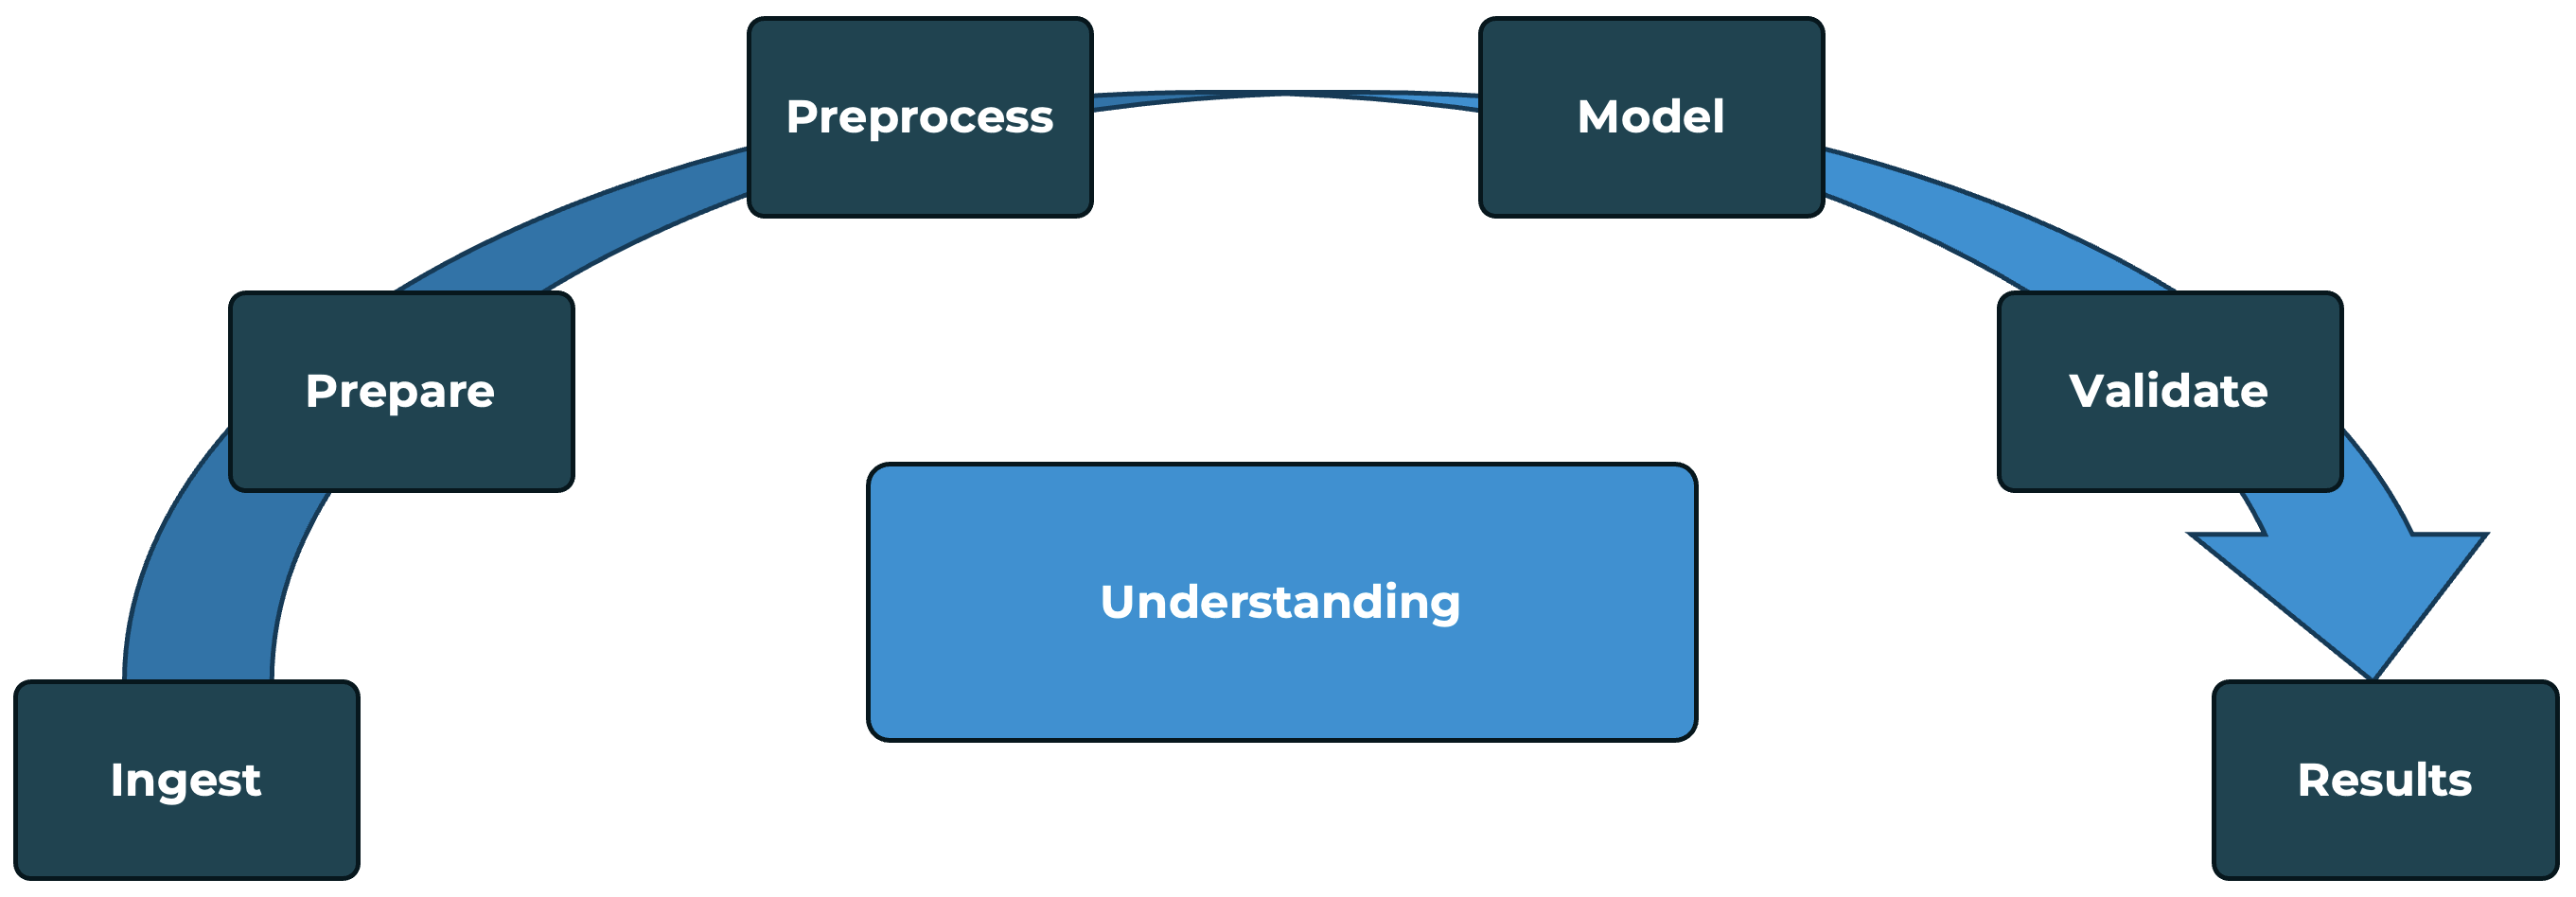
\includegraphics[width=0.9\textwidth]{fig_DS_Process.png}
\caption{\textbf{Core Data Science Process.} The process used in this paper consists of idempotent process steps of Ingest, Prepare, Pre-process, Model, and Validate.}
\end{figure}

\subsection{Ingesting Source Data}
Data ingestion was a manual process where individual documents were downloaded from web hosted repositories. File names included tags for specific metadata which was then used in follow on processes. Metadata in file names consisted of: publication year, document category, and publication type which was encoded into the file names to enable accurate processing. For example file \texttt{2001-DS-Astrophysics-9839.pdf} contains year (2001), corpus (DS), publication type (Astrophysics), and original document number (9839). These variables were chosen to enable follow on processes to identify corpus, place documents in chronological order, and retain publication type.  For information on the specific data used see Section~\ref{data} Data.

\subsection{Preparing the Text}
The first step in preparation is to extract the text from the PDF files. We completed this step with \texttt{PDFminer} which is a common PDF parser and analyzer\cite{pdfminer}. \texttt{PDFminer} extracted raw page text which is then cleaned with Python's \texttt{re} module which provides support for regular expressions and conducts find and replace operations on corpus text. Regular expressions were used to remove patterns in text such as special characters used in PDF formatting, page numbers, and blank pages. Document metadata, such as year of publication, was then extracted from the file names and stored as metadata with text from each page resulting in a total corpus size of just over 800 pages of NASA science plans and Decadal Surveys. Each page of clean text with metadata was then stored for further preprocessing with context embeddings. 

\subsection{Pre-processing with Context Embeddings}

Once the text is prepared each individual page is turned into a contextual embedding vector with 1536 dimensions using the \texttt{text-embedding-ada-002} model. High dimensional embeddings were chosen to leverage prior studies on document level search \cite{Aperdannier2024_embedding_search} and because we speculate that higher dimensionality provides a larger capacity to represent information. A page of text tends to contain multiple distinct ideas.  Higher-dimensional vector space may allow the model to better represent the context, semantics, and syntactic meaning in a large chunk of text such as a page of a PDF document and prevent distinct ideas from getting aggregated into a generic average. 

\subsection{Modeling with Contextual Comparison}
All contextually embedded pages for each individual corpus are then concatenated into a single index where all pages from all documents in the corpus are included in a single index. In the same way a Bag of Words model\cite{harris1954} is a simple text representation that disregards word order and only accounts for how many times a word appears, this model could be viewed as a Bag of Pages model that disregards page order and only accounts for the similarity of each page to other pages in the corpus. Page order is disregarded and only similarity of each page to the rest of the pages in the corpus is modeled. 

In order to investigate the relationship between scientific consensus and NASA plans a sequential approach is used placing NSF Decadal Surveys as the upstream corpus and NASA Science Plans as downstream corpus. Although NASA is independent from the NSF, NASA science Plans should inherit information from Decadal Surveys. This creates directional flow where information from the upstream Decadal Survey corpus flows to the downstream NASA science plan corpus. This sequential flow establishes a baseline to quantitatively measure semantic alignment between established scientific consensus and agency execution.

The distance of science plan pages is measured from the centroid of the Decadal Survey corpus. This was necessary because any single Decadal Survey covers only one of the NASA Science Mission Directorates while NASA Science Plans cover all 5 Science Mission Directorates. A mean of the 2001-2007 Decadal Surveys was chosen as those Surveys cover 4 of the 5 SMDs. This eliminates Biological and Physical Sciences from the reference centroid because the first Decadal Survey for this SMD was not released until 2011. Including this Survey would cause 3 of the 9 NASA science plans to occur after the last document in the Decadal Survey corpus thereby causing temporal leakage. 

The sample of Decadal Surveys creates a baseline to observe semantic drift of NASA plans that happens after Decadal Surveys are published. Semantic drift is defined here as the rate of separation of one corpus of text from another over time. The Surveys used in this analysis along with the year published and corresponding NASA SMD Division the Survey relates to is shown in Table~\ref{tab:Decadals_used}. For a complete table of Surveys see \ref{app_Decadal_Surveys}.

Information flow is modeled by creating a baseline of upstream NSF Decadal Survey corpus documents. This baseline is computed by calculating the mean of page vectors constituting the upstream sample corpus.

Figure~\ref{fig_simple_context_dist} is a simplified representation of the contextual distance model used. $X_{1}$ and $X_{2}$ each represent abstract axes of semantic similarity used to compare the documents. This simplifies the high dimensionality space of 1532 dimensions into just two unitless axes in order to visualize the concept. 

\begin{figure}[H]
\centering

\includegraphics[width=0.7
\textwidth]{fig_simple_context_dist.png}
\caption{\textbf{Simplified Contextual Distance Model.} The variables $X_1$ and $X_2$ represent abstract axes of semantic similarity, simplifying the high-dimensionality space of 1532 dimensions into two unitless axes for visualization. Downstream corpora chunks are represented inside the oval highlight. The median of the upstream corpus is represented by the blue dot. Lines illustrate the semantic alignment between the upstream and downstream corpora. Closer downstream chunks have higher semantic alignment to the upstream median.}

\label{fig_simple_context_dist}
\end{figure}

The alignment of each page in the NASA plan is calculated from the median of the Decadal Survey sample corpus represented by the blue dot surrounded by multiple pages. Individual pages of NASA plans are represented by individual page icons in Figure~\ref{fig_simple_context_dist}. 

The distance between Decadal Survey and science plans is represented by the lines connecting the pages and is measured using cosine similarity. Cosine similarity measures the angular distance between word vectors to determine the alignment of each page to the Decadal Survey corpus. Measuring by angular distance inherently normalizes for the natural page length variation in the corpora insuring page size does not skew the alignment scores\cite{manning2008_introduction_ir}. Cosine similarity was used in the training of the original embeddings model\cite{neelakantan2022openAi_embeddings} which creates a geometric structure we can better map to using cosine similarity. A perfectly aligned page would have a distance of 0 and, correspondingly, a cosine similarity of 1.

%%%%%%%%%%%%%%%%%%%%%%%%%%%%%%%%%%%%%%%%%%%%%%%%%%%%%%%%%%%%%%%%%%%%%%%%%%%%%%%%%%%
% results
%%%%%%%%%%%%%%%%%%%%%%%%%%%%%%%%%%%%%%%%%%%%%%%%%%%%%%%%%%%%%%%%%%%%%%%%%%%%%%%%%%%
\section{Analysis and Results} 
\label{anal_results}
Figure~\ref{swarm_all} displays the analysis of semantic alignment between NASA science plans and Decadal Surveys. The analysis spans from 2007 to 2025. The x-axis displays the publication year of the science plans, while the y-axis shows alignment of science plans to the Decadal Survey median. Each point represents a page from a science plan and is color coded to distinguish SMD-led plans from NASA-led plans. Points closer to the x-axis have lower alignment to the Decadal Survey median. A solid line represents the median similarity over time to illustrate the overarching trend. 

Yearly median similarity has an estimated decline of -0.001 similarity units per year coresponding to an overall decline of -0.024 similarity units from 2007 to 2025. A one-sided permutation test indicates this is a true nonzero trend with over 95\% confidence ($p=0.024$). Bootstrap 95\% confidence intervals are negative for both the slope (-0.0024 to -0.0002) and total change (-0.043 to -0.004). A linear fit yields $R^2 = 0.494$ indicating around half of the variation in midian similarity can be explained by time. These results support a modest downward shift in median similarity over time.

\begin{figure}[H]
\centering
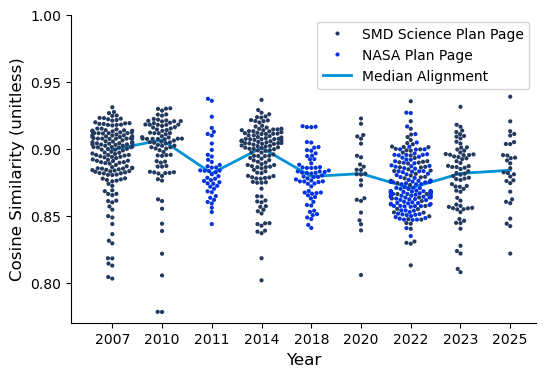
\includegraphics[width=0.9\textwidth]{SWARM_ALL.png}
\caption{\textbf{NASA Science Plan Similarity to Decadal Surveys.} Publication year is displayed on the x-axis and semantic aliment to the Decadal Survey median is measured on the y-axis. Single science plan pages are represented by individual points with color coding to distinguish SMD and NASA led plans. The solid line tracks the trend of median similarity over time. Points closer to the x-axis have lower alignment. One-sided permutation test ($p=0.024$) and bootstrap 95\% confidence intervals for slope (-.0024 to -0.0002) support a modest downward shift in median similarity over time.}\label{swarm_all}
\end{figure}

Figure~\ref{SWARM_SMD_vs_NASA} separates Science Mission Directorate led science plans from NASA led strategic plans. Pages in the corpus are once again represented by points on the graph and a median line is placed for each corpus subset. The SMD distribution is visibly shifted upward indicating a higher alignment with decadal surveys. The plotted median lines report a higher median for SMD Science plans ($0.895; n=551$) than for NASA Strategic Plans ($0.875; n=231$) with a difference of 0.020. A two-sided permutation test indicates the difference between medians is statistically significant ($p=9.9\times10^{-5}$) and a bootstrap 95\% confidence interval (0.016 to 0.025) excludes zero, supporting a significant difference between corpora. 

\begin{figure}[H]
\centering
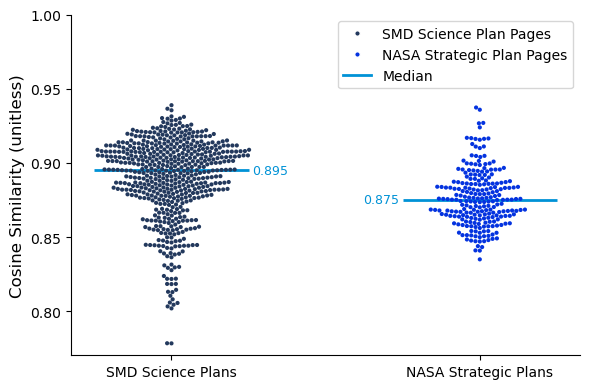
\includegraphics[width=0.9\textwidth]{SWARM_SMD_vs_NASA.png}
\caption{\textbf{NASA Science Mission Directorate and NASA Plans.} SMD alignment scores are shifted upward indicating SMD plans have a higher alignment with decadal surveys. SMD Science plans median (0.895; n=551) compared to NASA Strategic Plans median (0.875; n=231; $Delta=0.020$). The median difference is statistically significant at $p=9.9\times10^{-5}$ from a two-sided permutation test and bootstrap 95\% CI [0.016, 0.025].}\label{SWARM_SMD_vs_NASA}
\end{figure}

We can observe two patterns from Figure~\ref{swarm_all} and Figure~\ref{SWARM_SMD_vs_NASA}. First the median similarity of the NASA plans in relation to Decadal Surveys is decreasing over time. Second there is a difference between NASA led plans and SMD led plans. SMD led plan pages tend to be closer to the Decadal Survey median.
%%%%%%%%%%%%%%%%%%%%%%%%%%%%%%%%%%%%%%%%%%%%%%%%%%%%%%%%%%%%%%%%%%%%%%%%%%%%%%%%%%%
% Discussion
%%%%%%%%%%%%%%%%%%%%%%%%%%%%%%%%%%%%%%%%%%%%%%%%%%%%%%%%%%%%%%%%%%%%%%%%%%%%%%%%%%%
\section{Discussion and Future Work}
\label{discussion}

The decreased alignment over time between NASA plans and Decadal Surveys likely has many causal factors. In addition to Decadal Surveys NASA must have many other competing influences in science plans. We can conjecture that the decreased alignment may be a result of changes in consensus as Surveys are updated, changes in executive branch priorities, changes in congressional funding, or changes in operational realities. This introduces multiple vectors that are not accounted for in an analysis that focuses only on Decadal Surveys alignment to science plans. The difference in median alignment of SMD Science Plans and NASA Strategic plans is potentially the result of an increased effect from these unaccounted for vectors. The limited amount of data due to the once a decade periodicity of Survey publication limits the conclusions that can be drawn and ultimately provides analogous results. 

The alignment analysis conducted here suggests that measuring the change in semantic similarity is a useful methodology and highlights several areas for further study. This particular study could be expanded by categorizing Decadal Surveys into the 5 SMD divisions and exploring a more fine grained analysis of each scientific community. As a general approach, cross corpus contextual similarity analysis may be useful in other other areas where cross organizational alignment is a concern.  The approach could be extended by comparing page level, or smaller pieces of text across corpora by means of clustering algorithms. Optimization of architecture could also be explored by optimizing for embeddings models and hyperparameters.

%%%%%%%%%%%%%%%%%%%%%%%%%%%%%%%%%%%%%%%%%%%%%%%%%%%%%%%%%%%%%%%%%%%%%%%%%%%%%%%%%%%
% appendix
%%%%%%%%%%%%%%%%%%%%%%%%%%%%%%%%%%%%%%%%%%%%%%%%%%%%%%%%%%%%%%%%%%%%%%%%%%%%%%%%%%%
\newpage 
\appendix
\section{Complete List of Decadal Surveys}
\label{app_Decadal_Surveys}
A complete list of Decadal Surveys is given in Table \ref{tab:Decadals_all}. The table also incudes a Lessons Learned and Best Practices report conducted as a review of Decadal Surveys conducted in 2015. For researchers interested in learning more about this is a great resource \cite{Academies2015_lessons}.

\begin{table}[H]
\centering
\begin{tabular}{p{1.2cm} p{8.5cm} p{2.9cm}}
 \hline
 \rowcolor[gray]{0.95}
 \textbf{Year} & \textbf{Title} & \textbf{Corresponding SMD Division} \\

 1964 & Ground-based Astronomy a Ten-Year Program & Astrophysics \\

 1973 & Astronomy and Astrophysics for the 1970s & Astrophysics \\

 1982 & Astronomy and Astrophysics for the 1980s & Astrophysics \\

 1991 & A Decade of Discovery in Astronomy and Astrophysics & Astrophysics \\

 2001 & Astronomy and Astrophysics for the New Millennium & Astrophysics \\

 2003 & The Sun to the Earth—and Beyond: A Decadal Research Strategy in Solar and Space Physics & Heliophysics \\

 2003 & New Frontiers in the Solar System: An Integrated Exploration Strategy & Planetary Science \\

 2007 & Earth Science and Applications from Space: National Imperatives for the Next Decade and Beyond & Earth Science \\

 2010 & New Worlds, New Horizons in Astronomy and Astrophysics & Astrophysics \\

 2011 & Recapturing a Future for Space Exploration: Life and Physical Sciences Research for a New Era (2011) & Biological and Physical Sciences \\

 2011 & Vision and Voyages for Planetary Science in the Decade 2013-2022 & Planetary Science \\

 2013 & Solar and Space Physics: A Science for Technological Society & Heliophysics \\

 2015* & The Space Science Decadal Surveys: Lessons Learned and Best Practices (2015) & N/A \\

 2018 & A Midterm Assessment of Implementation of the Decadal Survey on Life and Physical Sciences Research at NASA (2018) & Planetary Science \\

 2018 & Thriving on Our Changing Planet: A Decadal Strategy for Earth Observation from Space & Earth Science \\

 2023 & Pathways to Discovery in Astronomy and Astrophysics for the 2020s (2023) & Astrophysics \\

 2023 & Thriving in Space: Ensuring the Future of Biological and Physical Sciences Research: A Decadal Survey for 2023-2032 (2023) & Biological and Physical Sciences \\

 2023 & Origins, Worlds, and Life: A Decadal Strategy for Planetary Science and Astrobiology 2023-2032 (2023) & Planetary Science \\

\end{tabular}
\caption{NASA Science Mission Directorate Decadal Surveys}\label{tab:Decadals_all}
\end{table}

\section{File Name Metadata}
\label{app_file_names}
This section details the file name convention used in this analysis and is provided to aid in future work. It is available at TODO: PUBLIC REPO. 

\begin{description}
 \item[Decadal file names:] Follow a \texttt{yyyy-DS-Category-\#\#\#\#.pdf} format where \texttt{\#\#\#\#} is the National Academies document number. \texttt{DS} is used to categorize all Decadal Surveys. \texttt{MA} replaces \texttt{DS} for Midterm Assessments, and \texttt{SP} is used for the Special Publication in 2015 that identified lessons learned.
 
 \item[Science plan file names:] Follow a \texttt{yyyy\_SSP\_Nasa\_File\_Name.pdf} format. \texttt{SSP} represents Science mission directorate Science Plans. This is replaced with \texttt{AD} to indicate Additional Documentation, \texttt{NSP} to indicate NASA Science Plan, or \texttt{AD} to indicate additional documentation present on the SMD website.
\end{description} 




%% Bibliography
\bibliographystyle{elsarticle-num} 
\bibliography{master.bib}

\end{document}


\endinput
%%
%% End of file `elsarticle-template-num.tex'.

\section{BEGIN Template Sections }
\label{sec1}
%% Labels are used to cross-reference an item using \ref command.

Section text. See Subsection \ref{subsec1}.


%% Use \subsection commands to start a subsection.
\subsection{Example Subsection}
\label{subsec1}

Subsection text.

%% Use \subsubsection, \paragraph, \subparagraph commands to 
%% start 3rd, 4th and 5th level sections.
%% Refer following link for more details.
%% https://en.wikibooks.org/wiki/LaTeX/Document_Structure#Sectioning_commands

\subsubsection{Mathematics}
%% Inline mathematics is tagged between $ symbols.
This is an example for the symbol $\alpha$ tagged as inline mathematics.

%% Displayed equations can be tagged using various environments. 
%% Single line equations can be tagged using the equation environment.
\begin{equation}
f(x) = (x+a)(x+b)
\end{equation}

%% Unnumbered equations are tagged using starred versions of the environment.
%% amsmath package needs to be loaded for the starred version of equation environment.
\begin{equation*}
f(x) = (x+a)(x+b)
\end{equation*}

%% align or eqnarray environments can be used for multi line equations.
%% & is used to mark alignment points in equations.
%% \\ is used to end a row in a multiline equation.
\begin{align}
 f(x) &= (x+a)(x+b) \\
   &= x^2 + (a+b)x + ab
\end{align}

\begin{eqnarray}
 f(x) &=& (x+a)(x+b) \nonumber\\ %% If equation numbering is not needed for a row use \nonumber.
   &=& x^2 + (a+b)x + ab
\end{eqnarray}

%% Unnumbered versions of align and eqnarray
\begin{align*}
 f(x) &= (x+a)(x+b) \\
   &= x^2 + (a+b)x + ab
\end{align*}

\begin{eqnarray*}
 f(x)&=& (x+a)(x+b) \\
   &=& x^2 + (a+b)x + ab
\end{eqnarray*}

%% Refer following link for more details.
%% https://en.wikibooks.org/wiki/LaTeX/Mathematics
%% https://en.wikibooks.org/wiki/LaTeX/Advanced_Mathematics

%% Use a table environment to create tables.
%% Refer following link for more details.
%% https://en.wikibooks.org/wiki/LaTeX/Tables
\begin{table}[t]%% placement specifier
%% Use tabular environment to tag the tabular data.
%% https://en.wikibooks.org/wiki/LaTeX/Tables#The_tabular_environment
\centering%% For centre alignment of tabular.
\begin{tabular}{l c r}%% Table column specifiers
%% Tabular cells are separated by &
 1 & 2 & 3 \\ %% A tabular row ends with \\
 4 & 5 & 6 \\
 7 & 8 & 9 \\
\end{tabular}
%% Use \caption command for table caption and label.
\caption{Table Caption}\label{tab1}
\end{table}


%% Use figure environment to create figures
%% Refer following link for more details.
%% https://en.wikibooks.org/wiki/LaTeX/Floats,_Figures_and_Captions
\begin{figure}[t]%% placement specifier
%% Use \includegraphics command to insert graphic files. Place graphics files in 
%% working directory.
\centering%% For centre alignment of image.
\includegraphics{example-image-a}
%% Use \caption command for figure caption and label.
\caption{Figure Caption}\label{fig1example}
%% https://en.wikibooks.org/wiki/LaTeX/Importing_Graphics#Importing_external_graphics
\end{figure}
